% Author: Till Tantau
% Source: The PGF/TikZ manual
\documentclass{article}

\usepackage{tikz}
\usepackage{verbatim}

\begin{document}
\pagestyle{empty}

\begin{comment}
:Title: Maze
:Tags: Manual, Paths

This example is from the utilities page of the TikZ and PGF manual.

| Author: Till Tantau
| Source: The PGF/TikZ manual

\end{comment}

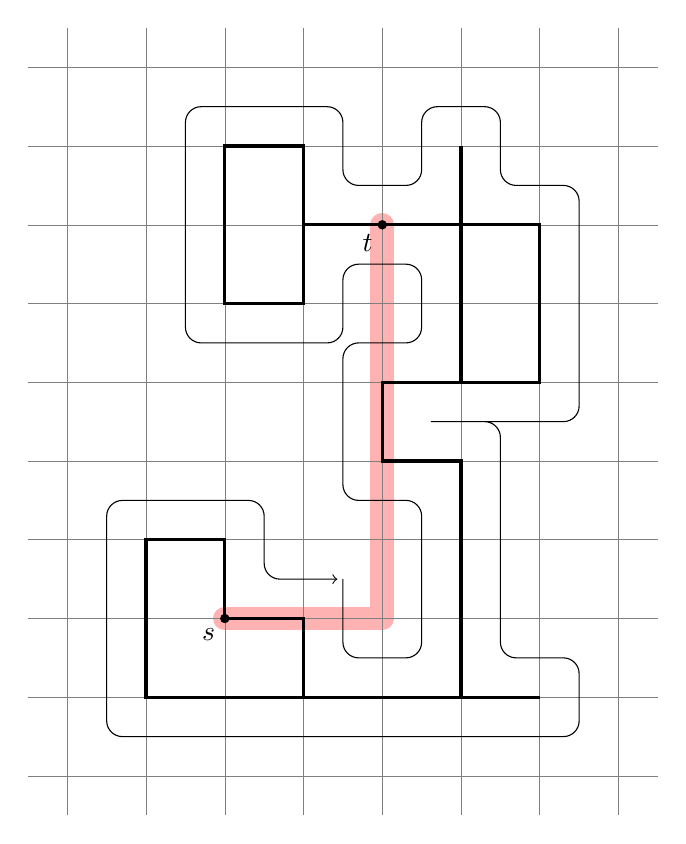
\begin{tikzpicture}
  \draw[line width=0.3cm,color=red!30,cap=round,join=round] (0,0)--(2,0)--(2,5);
  \draw[help lines] (-2.5,-2.5) grid (5.5,7.5);
  \draw[very thick] (1,-1)--(-1,-1)--(-1,1)--(0,1)--(0,0)--
    (1,0)--(1,-1)--(3,-1)--(3,2)--(2,2)--(2,3)--(3,3)--
    (3,5)--(1,5)--(1,4)--(0,4)--(0,6)--(1,6)--(1,5)
    (3,3)--(4,3)--(4,5)--(3,5)--(3,6)
    (3,-1)--(4,-1);
  \draw[below left] (0,0) node(s){$s$};
  \draw[below left] (2,5) node(t){$t$};
  \fill (0,0) circle (0.06cm) (2,5) circle (0.06cm);
  \draw[->,rounded corners=0.2cm,shorten >=2pt]
    (1.5,0.5)-- ++(0,-1)-- ++(1,0)-- ++(0,2)-- ++(-1,0)-- ++(0,2)-- ++(1,0)--
    ++(0,1)-- ++(-1,0)-- ++(0,-1)-- ++(-2,0)-- ++(0,3)-- ++(2,0)-- ++(0,-1)--
    ++(1,0)-- ++(0,1)-- ++(1,0)-- ++(0,-1)-- ++(1,0)-- ++(0,-3)-- ++(-2,0)--
    ++(1,0)-- ++(0,-3)-- ++(1,0)-- ++(0,-1)-- ++(-6,0)-- ++(0,3)-- ++(2,0)--
    ++(0,-1)-- ++(1,0);
\end{tikzpicture}

\end{document}